%!TEX root = ../thesis.tex
\newchap{Event classification and signal extraction}\label{sec:signal}
\vspace{-1cm}
\minitoc
This chapter is focused on the signal-background discrimination. It will begin by demonstrating a basic one-dimensional feature ranking. Subsequently, JPANet will be adapted to tackle the signal-background discrimination challenge, and its score will be employed to execute a template fitting procedure on both the Muon and Electron channels, utilizing the Asimov dataset.
Once the statistical uncertainties associated with the $\PW \to cb$ rate are determined, we will also introduce and assess the systematic uncertainties and their impact on the signal rate extraction.
\TODO{Aggiungi roba quando fai il ratio}\\
\begin{minipage}[H]{\linewidth}
\begin{minipage}{0.35\linewidth}
        \centering
        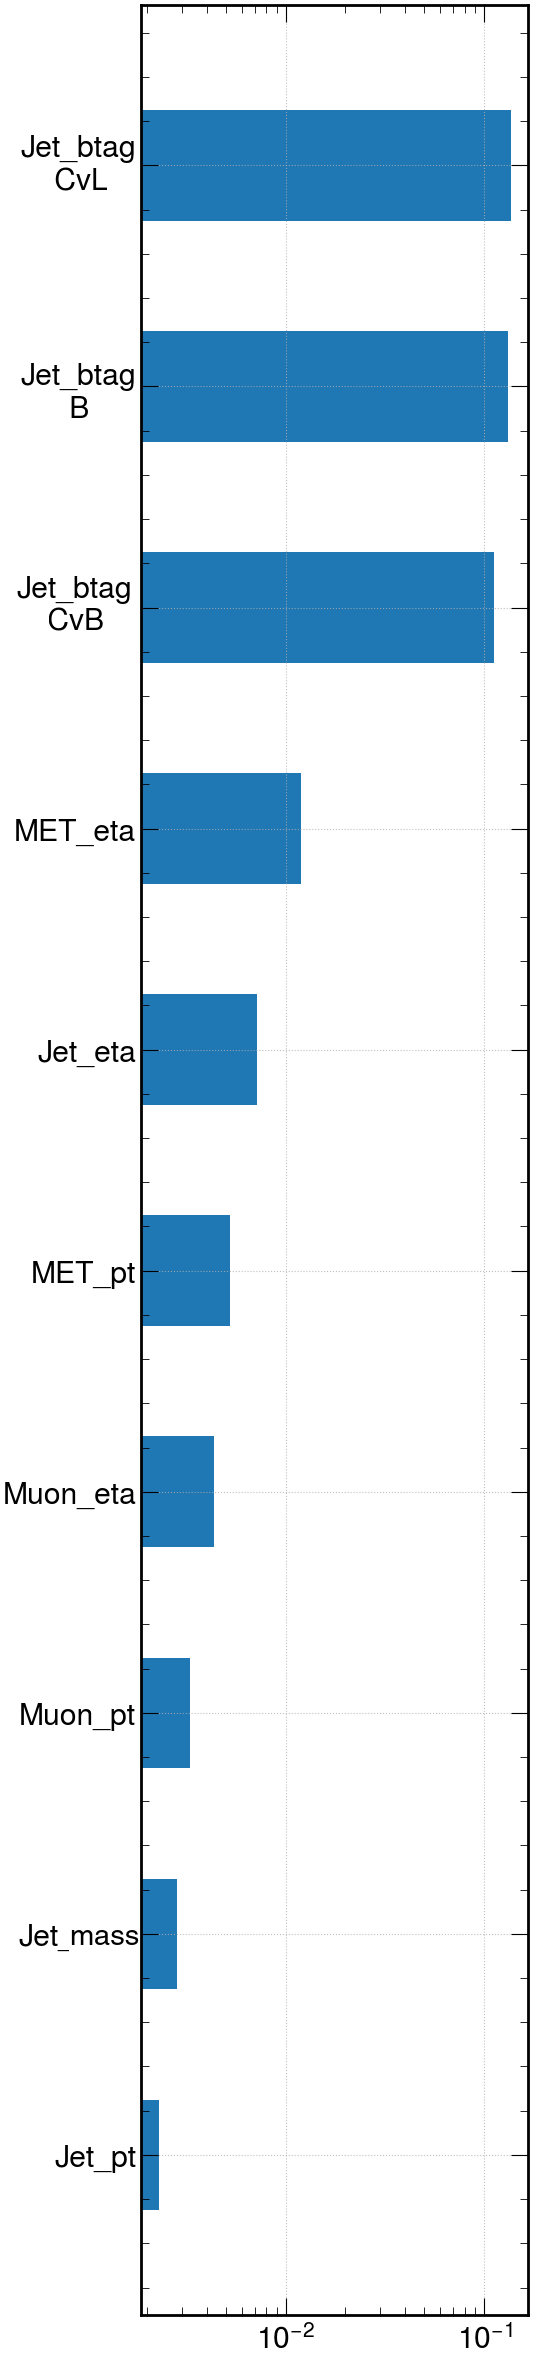
\includegraphics[height=0.7\textheight]{fig//chap08-kin_reco/ranking1D.png}
        
\end{minipage}
\hfill
\begin{minipage}{0.62\linewidth}
\vspace{-1cm}
\section{Unidimensional feature ranking}
To begin,  we can once again employ the metric $d$ to evaluate and rank the observables that discriminate the signal from the background.\\
\\
In this context, $d$ is computed between the signal and the $\ttbar$ semileptonic process, which is the primary source of background.\\
\\
All observables are treated as flattened, meaning that all objects within the events are combined in the same histograms, disregarding the event's inherent structure.\\
\\
The ranking process is carried out within the Muon channel following the initial preselection.\\
The results of this one-dimensional ranking are depicted in \Fig{fig:1Drank}.\\
\\
Notably, the observables with the highest ranking are those associated with b-tagging, exhibiting $d$ values of approximately 0.1.\\
Meanwhile, other observables produce results that are about an order of magnitude smaller, and the latests are due mostly to statistical fluctuations.

\end{minipage}
        \label{fig:1Drank}  
        \captionof{figure}{Unidimensional feature ranking using the metric $d$ between flattened signal observables and \ttbar semileptonic observables }
\end{minipage}
\section{Event classification}
\paragraph*{SBANet} Since we have already demonstrated the ability of JPANet to reconstruct and interpret the signal events, we can exploit the same model to tackle the signal-background discrimination task.\\
To do it we have just to introduce some modifications into JPANet, creating another network which will be denoted as "Signal-Background Attention Network" (SBANet).\\
This network will be trained and evaluated separately in the Muon and Electron channels.\\
\\
The differences between SBANet and JPANet are:
\\
\textbf{Jet Inputs}: In SBANet, all the three \DeepJet scores are added to the Jet head (b-tag,CvB,CvL).
\\
\\
\textbf{Hyper-parameters}: Doing some trials it was proven that the network needed to be more complex, so the number of units of each feed-forward layer was increased to 128 and the dropout probability to 2\%.
\\
\\
\textbf{Self-attention pooling}: The output of JPANet is a matrix $7 \times 4$ because we have to assign a score to each pair of jet-partons, but now we have to assign a single score to the event.\\
To do it we have to reduce the jet embedding sequence to just one dimension. This was done using a self-attention pooling layer that weights each element of the sequence (\ie the physics objects) with the attention scores and performs a weighted average of the embedding sequence across the sequence.\\
Subsequently, three feed-forward were added.  
\\
\\
\textbf{Event self-attention}: We want the self-attention pooling to compute the attention scores over all the physics objects and not just on the jets, so the JPANet cross-attention was turned in a self-attention over the concatenated sequence of the jets and of the leptonic W.
\\
\\
\textbf{Output layer} The output of SBANet is a 3-dimensional layer equipped with the softmax function. Three classes are defined: the signal, the $\ttbar$ semileptonic process, and the $\ttbar$ dileptonic process. In this way, we can train the network to better distinguish the signal from the two main populated sources of background, also if, in the end, we will consider just the signal score.
\\  
\\
\textbf{Secondary leptons head} Another minimal head was added to help SBANet to recognize di-leptonic events. This head, in the muon(electron) channel, is composed of a sequence of 3 elements: the second leading muon(electron), and the leading and the second leading electrons(muons).\\
The lepton features are just the kinematic variables $(p_T,\eta,\phi)$ and the head is connected to a 2-layer feed-forward neural network.\\
The secondary leptons embedding sequence is then concatenated to the full event sequence before the self-attention pooling layer.
\\
\\
\textbf{Invariant mass heads and pair-wise attention biases} The two self-attention layers in the network were modified to include pair-wise physics object features, like invariant masses.\\
Let's recall what the self-attention is:
\begin{equation}
    \text{Softmax}\left( \frac{QK}{d_k} \right)V
\end{equation}
The product $QK$ is a $N\times N$ matrix where N is the length of the sequence.\\
Given that we can include the invariant masses of couples of physics objects by just adding a term in the softmax function
\begin{equation}
    \text{Softmax}\left( \frac{QK+\hat{M}}{d_k} \right)V
\end{equation}
where $\hat{M}$ is a linear embedding of the matrix $M$ that contains all the invariant masses
\begin{equation}
\begin{aligned}
    M_{ij}&=\sqrt{(p_i+p_j)^\mu(p_i+p_j)_\mu} & \text{if } i\neq j\\
    M_{ij}&=m_i & \text{if } i=j\\
\end{aligned}
\end{equation}
The M matrix is symmetric and has $N(N+1)/2$ independent components. The strategy to implement this in SBANet is adding another head containing for each event a vector of length 36 with the square invariant masses of the couple of jets and the leptonic W.
\begin{equation*}
    \text{Mass head inputs}=\Biggl[ \dboxed{m_W,m_{Wj_1},\dots,m_{Wj_7},\dboxed{m_{j_1},m_{j_1 j_2},\cdots,m_{j_2},m_{j_2 j_3},\cdots}}\: \Biggr]
\end{equation*}
This vector contains all the independent components of the M matrix.\\
Since the first self-attention layer works only on the jet sequence and the other on the jet + leptonic W sequence, we have to build two different mass embeddings.\\
\\
For jet-self attention, only the mass inputs that are not related to the leptonic W boson are considered. They are 28 elements that are fed to a 4-layer feed-forward neural network of size [28,128,128,28]. This network that has the same number of neurons in the first and the last layer is called Autoencoder.\\
The 28 output elements of the autoencoder are used to build the full $7\times 7$ M matrix that will be used as attention bias in the jet self-attention.\\
\\
The same thing is done with the event self-attention but considering all the mass head inputs and, in this case, the autoencoder size will be [36,128,128,36]


%Scrivi i datasets, cross entropy reweighted


%loss




\section{Signal rate extraction}
\subsection{Systematic uncertainties}
\section{Ratio extraction}
\subsection{Systematic uncertainties}